\chapter{FPGA Design \& Implementation} 
% architecutr &design & impementation
\label{Chapter-FPGA-Implementation}

\section{Tools Used}
\subsection{Vitis Unified Software Platform}
The Vitis unified software platform\cite{Vitis_unified_software_platform} is a collection of tools, libraries and environments designed to ease the development of accelerated applications tailored for AMD Xilinx FPGA and Versal® ACAP hardware platforms. It includes graphical and command-line compilers, analyzers, and debuggers to build applications, analyze performance bottlenecks, and debug accelerated algorithms, developed in C, C++, or OpenCL APIs. Furthermore, it offers numerous advantages such as effortless application portability, complete simulation of hardware systems, and an open source runtime that handles host-device communication.
\begin{figure}[H]
    \centering
        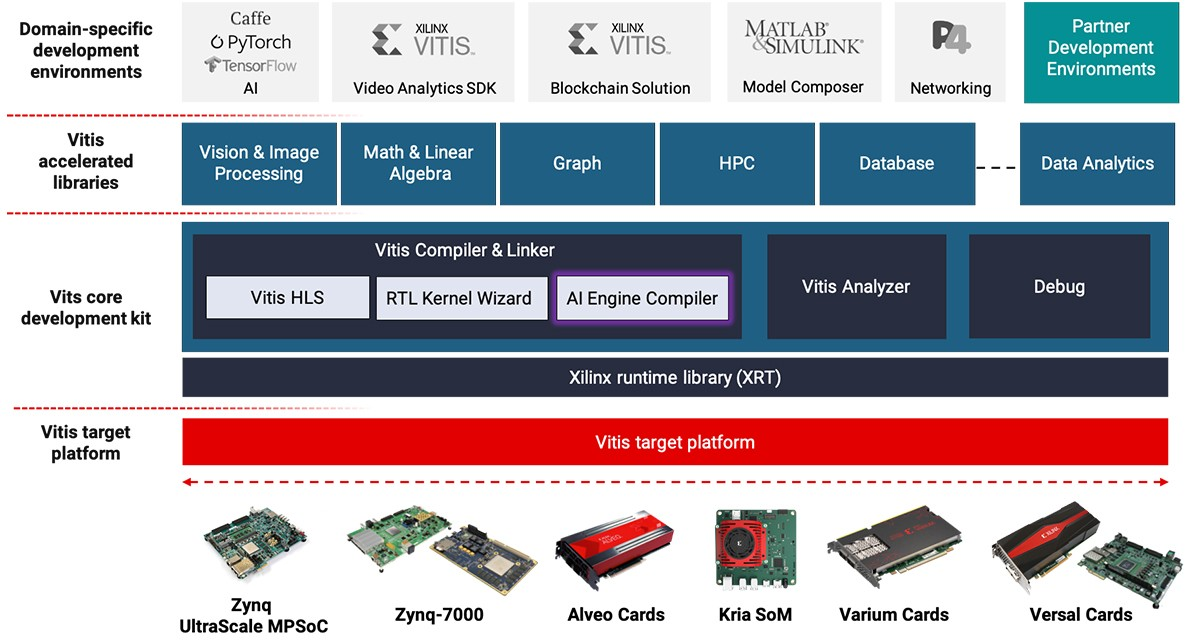
\includegraphics[width=1\textwidth]{Images/Platform/vitis.jpg}
        \decoRule
        \caption[Vitis]{Vitis overview: \href{https://www.xilinx.com/products/design-tools/vitis/vitis-platform.html\#overview}{URL}.}
        \label{fig:Vitis_overview}
\end{figure}

Vitis supports hardware acceleration kernels controlled by PS or x86 kernels. The Vitis application acceleration development flow provides a framework for developing and delivering FPGA-accelerated applications using standard programming languages for both software and hardware components. The kernels can be developed through traditional RTL, C/C++ with Vitis HLS, the Vitis model composer and the AI Engine compiler.
\begin{figure}[H]
    \centering
        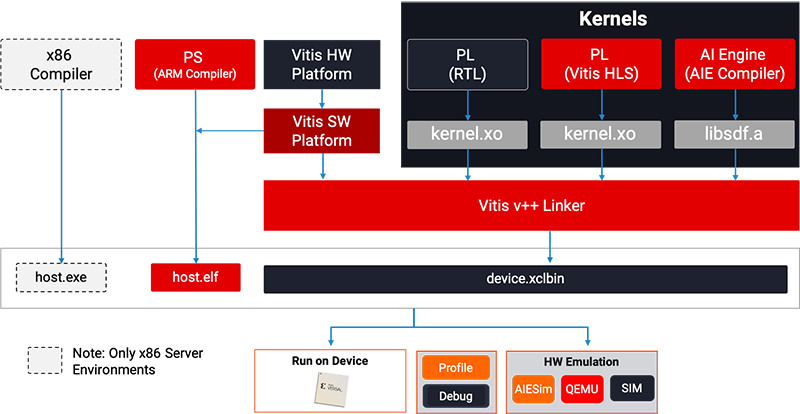
\includegraphics[width=1\textwidth]{Images/Platform/vitis_kernel.png}
        \decoRule
        \caption[Vitis]{Vitis kernel architecture: \href{https://www.xilinx.com/products/design-tools/vitis/vitis-platform.html\#development}{URL}.}
        \label{fig:Vitis_kernel_overview}
\end{figure}

\subsection{Xilinx Runtime library (XRT)}
The Xilinx Runtime library\cite{Xilinx_Runtime_Library} (XRT) facilitates communication between the application code (running on an embedded Arm or x86 host) and the accelerators deployed on the reconfigurable portion of PCIe interface-based AMD Xilinx accelerator cards, MPSoC-based embedded platforms, or ACAPs. It is flexible with modifiable libraries and drivers, enabling different levels of abstractions, from high-level Python bindings to low-level C++ APIs. Its APIs are common across all platforms and require no hardware expertise, eliminating the need to implement hardware communication layers from scratch.
\begin{figure}[H]
    \centering
        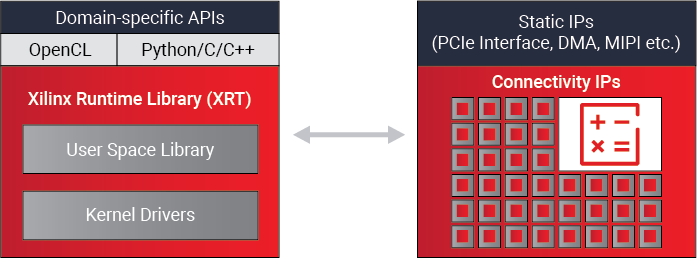
\includegraphics[width=1\textwidth]{Images/Platform/xrt.png}
        \decoRule
        \caption[Xilinx Runtime Library]{Xilinx Runtime Library overview: \href{https://www.xilinx.com/products/design-tools/vitis/xrt.html}{URL}.}
        \label{fig:XRT_overview}
\end{figure}

\subsection{Vitis High Level Synthesis (HLS)}
The Vitis HLS tool can synthesize a C/C++ function into RTL code for implementation in the programmable logic (PL) region of a Xilinx FPGA device. Its kernels can be easily integrated into a design utilizing OpenCL\cite{OpenCL} code. It provides support of complex data types, math functions and AXI4-Stream interfaces for data exchange between IPs in the PL and/or Processing Subsystem (PS).

HLS is an automated design process that takes an abstract behavioral specification of a digital system and generates a register-transfer level structure that implements the given behavior. The designer is working on a high abstraction level, while the tool takes care of mechanical RTL implementation tasks.

\begin{table}[H]
    \center
    \begin{tabular}{ | c | }
        \hline
        Designer's Responsibilities\\
        \hline
        Macro Architecture\\
        Design Intent\\
        Constrains\\
        \hline
        \multicolumn{1}{ c }{ } \\
        \multicolumn{1}{ c }{ } \\
        \multicolumn{1}{ c }{ } \\
        \multicolumn{1}{ c }{ } \\
    \end{tabular}
    \quad
    \begin{tabular}{ | c | }
        \hline
        HLS tool automation\\
        \hline
        FSM Generation\\
        Operation Scheduling\\
        Clock\\
        Register Pipelining\\
        Resource Sharing\\
        Timing\\
        Verification\\
        \hline
    \end{tabular}
    \caption[HLS responsibilities]{Distribution of work during HLS design.}
    \label{HLS responsibilities}
\end{table}

\section{FPGA Platforms}

\subsection{Xilinx Zynq UltraScale+ MPSoC}
The Zynq\textsuperscript{\textregistered} UltraScale+\texttrademark{} MPSoC is a family of Xilinx products that integrates a feature-rich 64-bit quad-core or dual-core Arm® Cortex®-A53 and dual-core Arm Cortex-R5F based processing system (PS) and Xilinx programmable logic (PL) UltraScale architecture in a single device. In addition, on-chip memory, multiport external memory interfaces, and a rich set of peripheral connectivity interfaces are included. \cite{Zynq_UltraScale_overview}

\subsection{ZCU102 Evaluation Board}
The ZCU102 Evaluation Board features a Zynq\textsuperscript{\textregistered} UltraScale+\texttrademark{} MPSoC with a quad-core Arm\textsuperscript{\textregistered} Cortex\textsuperscript{\textregistered}-A53, dual-core Cortex-R5F real-time processors, and a Mali\texttrademark{}-400 MP2 graphics processing unit based on Xilinx's 16nm FinFET+ programmable logic fabric. It supports all major peripherals and interfaces, enabling development for a wide range of applications. Furthermore, its high speed DDR4 memory interfaces, variety of communication interfaces and FMC expansion ports makes it ideal for rapid prototyping. 

\begin{figure}[H]
    \centering
        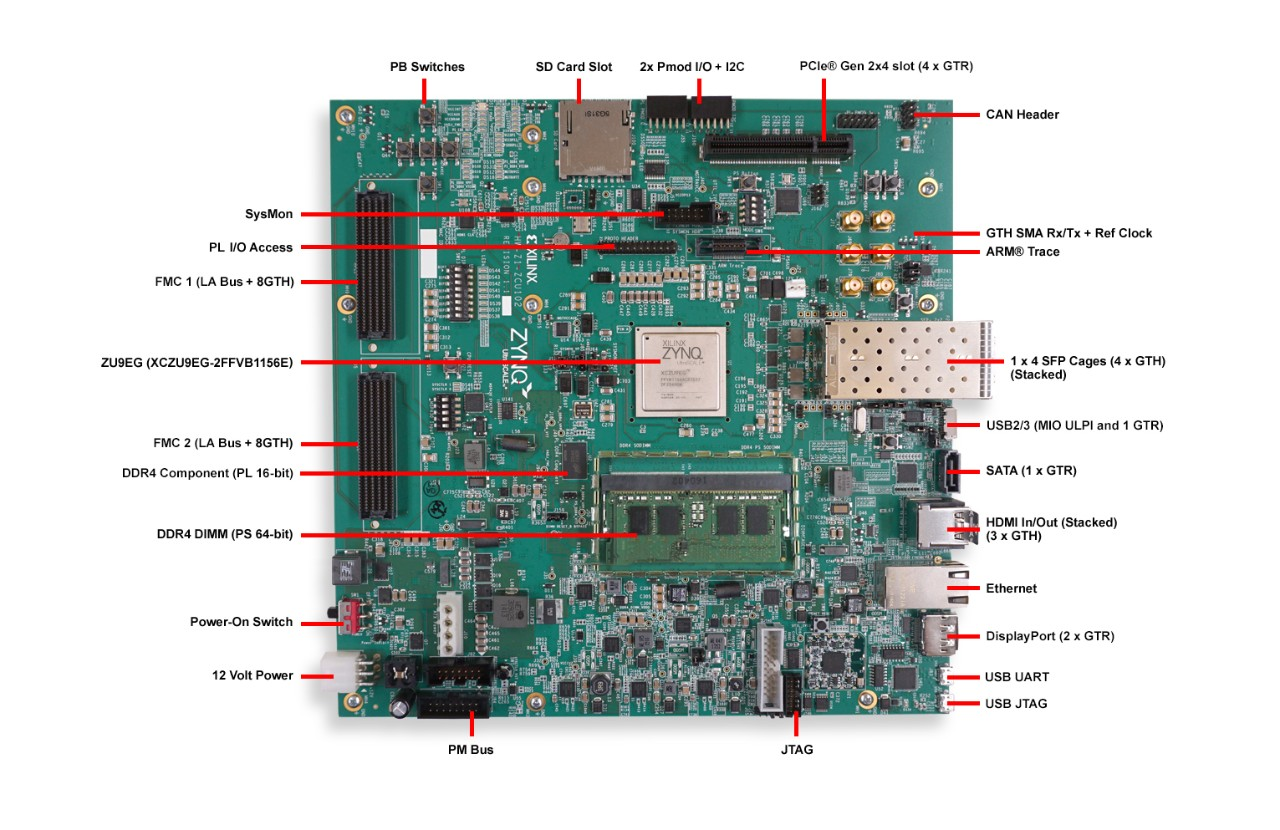
\includegraphics[width=1\textwidth]{Images/Hardware/zcu102.jpg}
        \decoRule
        \caption[ZCU102]{ZCU102 Features: \href{https://www.xilinx.com/products/boards-and-kits/ek-u1-zcu102-g.html\#information}{URL}.}
        \label{fig:ZCU102}
\end{figure}

Given that the thesis is based on an edge application, this platform seems to be an ideal fit for it. During the hardware design phase, the constrains and resource limitation were placed according to the specifications of this board. Nevertheless, transferring the final design to devices of similar families should require minimal effort.

\section{Hardware Implementation}

\subsection{C++ CNN Implementation}
During the preceding phase, TF with Python was utilized to implement all ANNs and training. Due to the Vitis Kernel Toolchain requires C/C++ code, these implementations can not be synthesized to hardware by the aforementioned tools. As such, the most used CNN, the third in the model library, has been re-implemented on C++.

Migrating from TF to a hardware synthesizable CNN is a fairly challenging task riddled with pitfalls. This implementation is not optimized for hardware, but rather serves as a stepping stone between TF and synthesizable code. Certain practices are adopted to facilitate future transition to hardware targeted code:

\begin{itemize}[leftmargin=*]
    \item Implementation is modular and re-configurable. The code is build around template functions, each of which performs a specified task. Layers can effortlessly added, removed, or altered in size, shape and parameters.
    \item All data, whether input, output or internal, are produced and consumed serially and only once. This behavior is similar to the stream data format, which is widely utilized in hardware design.
    \item All feature maps, input gradients, variable gradients, and updated variables are logged and compared with those generated by the existing TF implementation. This approach not only evaluates functionality, but also produces test benches for future hardware implementation.
\end{itemize}

\begin{figure}[H]
    \centering
        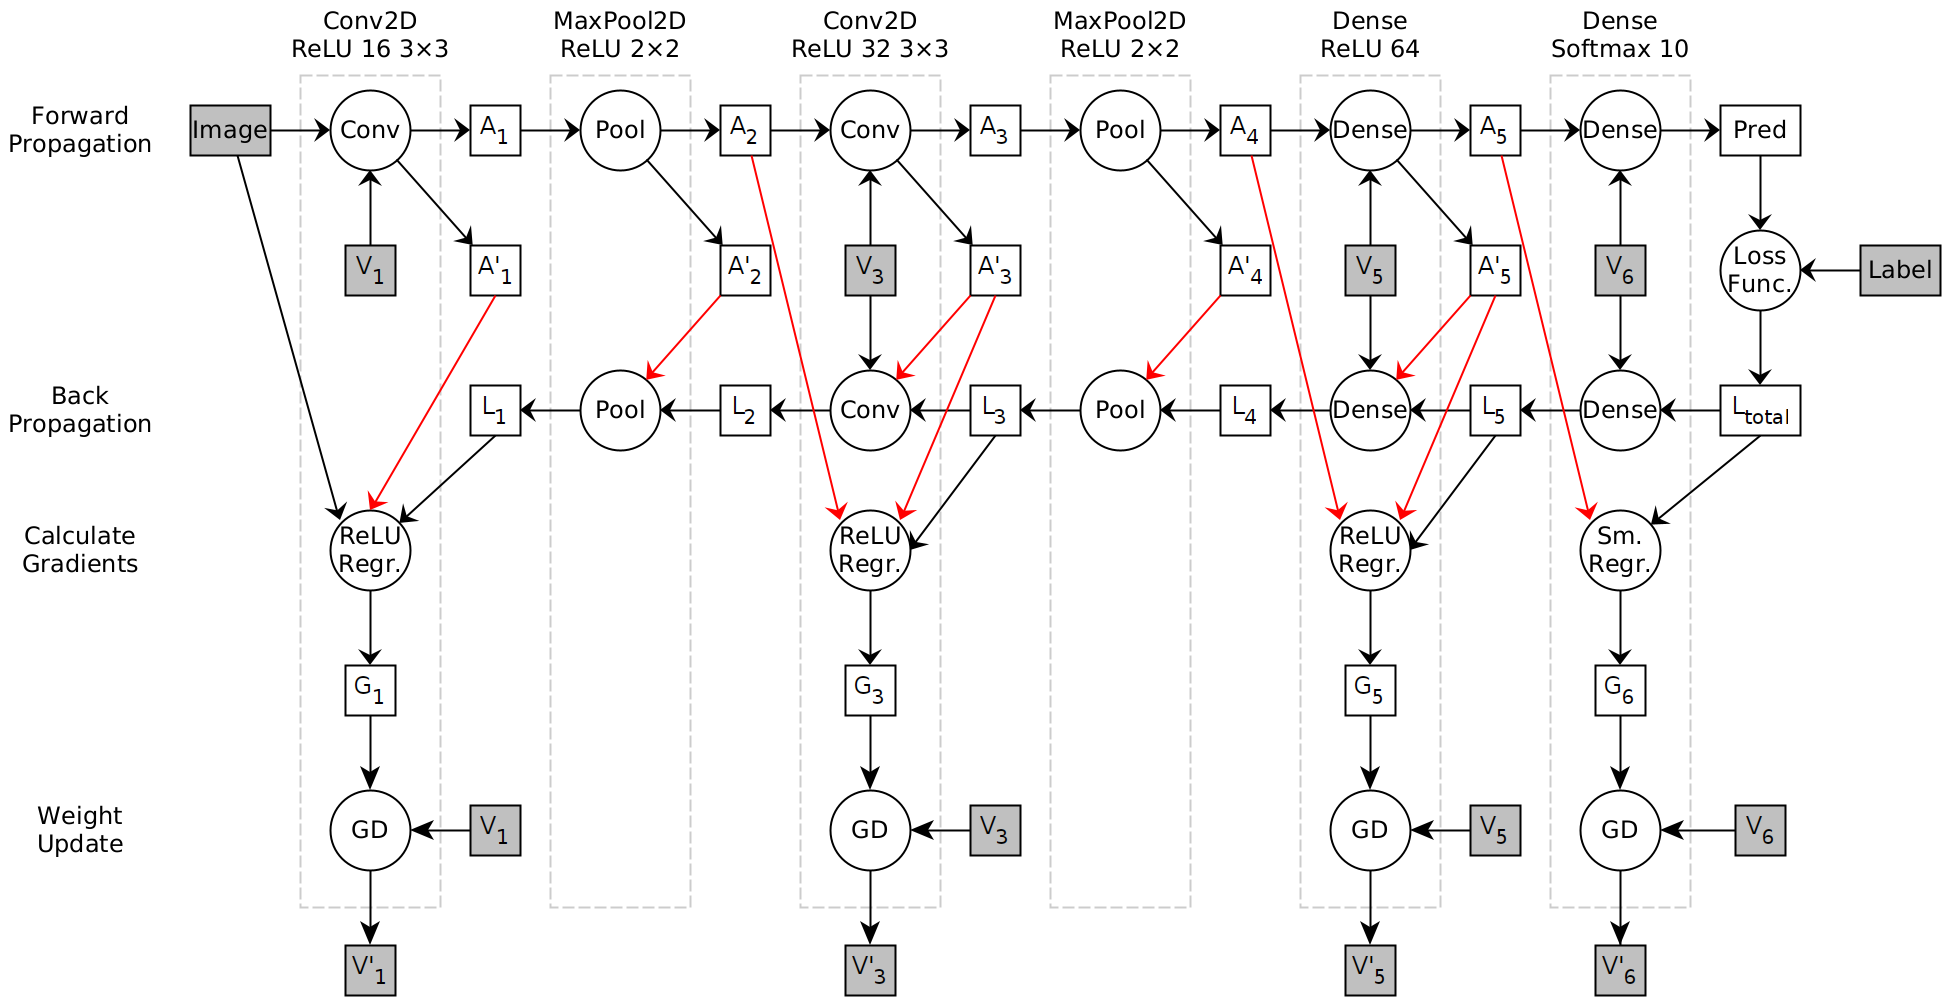
\includegraphics[width=1\textwidth]{Images/block_diagrams/dataflow_cnn_model.png}
        \decoRule
        \caption[CNN dataflow]{Dataflow diagram of the utilized CNN model.}
        \label{fig: CNN dataflow}
\end{figure}

Figure \ref{fig: CNN dataflow} depicts the basic structure of the implementation. Tasks are represented by cycles, whereas data are represented by squares. Inputs, labels, weights and any other data that must to be saved in memory have greyed-out squares. The majority of internal data are consumed immediately after being produced. Some of them, marked by red arrows, skip parts of the chain and must be temporally stored.

\subsection{Vitis HLS Implementation}
Even with the aforementioned techniques, adapting the code to be compatible with FPGAs is not a trivial task. To build an efficient implementation, resource usage, data access patterns, and other factors must be taken into account. All parts of the CNN are modified accordingly.

\subsubsection{2D Convolutional Layers}
Due to their non-serial data access patterns, multi-dimensional filter algorithms frequently conflict with FPGA design; 2-D convolution is no exception. At its core, it carries out some form of data averaging around a pixel, necessitating the access of nearby input values as seen in figure \ref{fig: convolution access pattern}. Additionally, when calculating the adjacent outputs, some inputs are accessed again.

\begin{figure}[H]
    \centering
        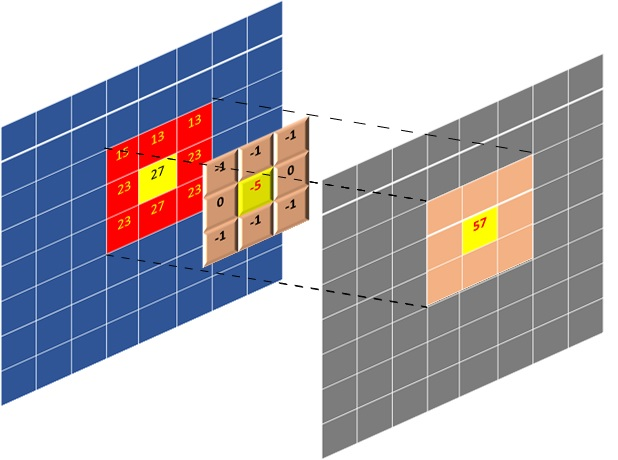
\includegraphics[width=1\textwidth]{Images/diagrams/convolution_access_pattern.jpg}
        \decoRule
        \caption[convolution access pattern]{Convolution access pattern: Input (Blue) pixels are accessed in a non-serial pattern.\href{https://github.com/Xilinx/Vitis-Tutorials/blob/2022.1/Hardware_Acceleration/Design_Tutorials/01-convolution-tutorial/lab1_app_introduction_performance_estimation.md}{URL} }
        \label{fig: convolution access pattern}
\end{figure}

In a CPU-focused implementation this would be a non issue, as data caching and pre-fetching can ensure that the majority of accesses will be cache hits. Implementing this on an FPGA would produce numerous small non-burst accesses on the global memory, resulting in unacceptable performance. Thus, a different approach is required.

A unique data mover, specifically designed for the given algorithm, has been developed to reduce the number of global memory accesses. Its key concept is to construct two-dimensional input windows that are the same size as the filters and then compute the dot product of those. Its main components are buffers that store lines of the input, and a sliding window on top of them.

\begin{figure}[H]
    \centering
        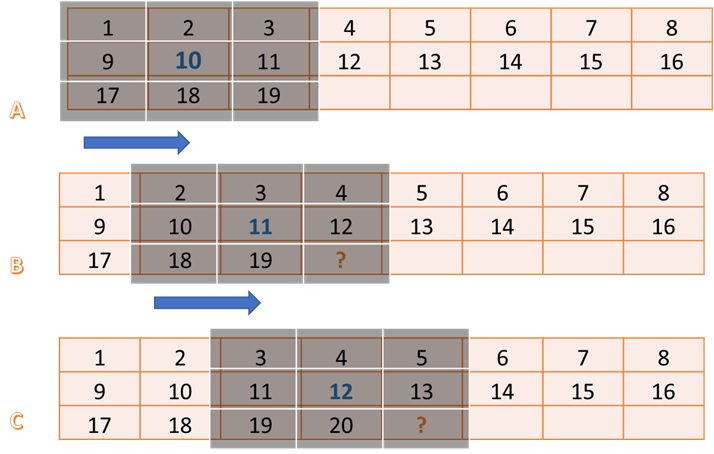
\includegraphics[width=1\textwidth]{Images/diagrams/line_buf_conv.jpg}
        \decoRule
        \caption[Line Buffers, Convolution]{Line Buffers: Sifting a 3x3 window. \href{https://github.com/Xilinx/Vitis-Tutorials/blob/2022.1/Hardware_Acceleration/Design_Tutorials/01-convolution-tutorial/lab2_conv_filter_kernel_design.md}{URL} }
        \label{fig: Line Buffers Convolution}
\end{figure}

Figure \ref{fig: Line Buffers Convolution} illustrates the operation of the line and window buffering scheme. A continuous stream of 3x3 windows is produced by sifting a window buffer over the top of the line buffers. Since the masked elements of the top line are already present in the window, only two line buffers are needed. More important observation is that only one new input pixel is required to produce a window, and thus an output pixel. Finally, zero padding is applied to maintain correct data with edge windows.

To complete the 2D convolution, a processing element is required. In the simplest scenario, a single channel input, the dot products between the windows and the filters are calculated and activated with the ReLU function. If there are additional input channels, the dot products are calculated in respect of each channel, which are aggregated and then activated to produce the feature map of the layer. This is done to allow computing of multiple channels in parallel, while using a data streaming paradigm.

\begin{figure}[H]
    \centering
        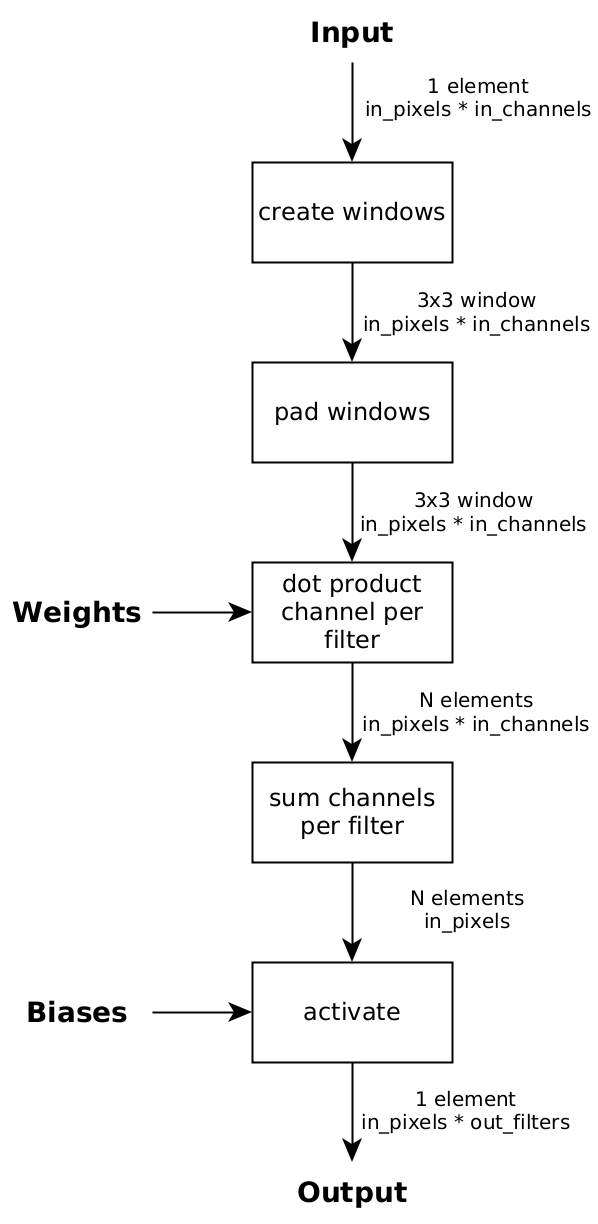
\includegraphics[width=0.5\textwidth]{Images/block_diagrams/conv2d_mc.png}
        \decoRule
        \caption[Conv2D block diagram]{Block diagram of the forward propagation for the 2D convolution. N is the number of filters. The data types of the internal streams with the total data passed are shown. }
        \label{fig: Conv2D block diagram}
\end{figure}

The overall scheme is designed to maximize the data reuse providing maximum parallel data to the processing element, with minimum use of memory. Back propagation and gradient calculation follow the same logic with a few minor differences:

In back propagation, the input is the activated output gradients. To activate them, the system need to remember which neurons fired during forward propagation, as shown in figure \ref{fig: CNN dataflow}. Furthermore, the biases are not used, and the channel/filter dimensions are reversed. Finally the output are the input gradients.

The processing element of the gradient calculation differs a bit more. Instead of using the weights to calculate the outputs, the outputs are used to calculate the weight gradients. Furthermore, finding the bias gradients is trivial, as they are equal with the sum of all output gradients of their filter.

\subsubsection{2D Max-Pooling Layers}
The 2D Max-Pooling layers are implemented using the same logic as the 2D convolutional layers, albeit with a few major differences. First of all the window is 2x2 is size, and with a stride of 2. As a result, each window contains exclusive data, and an output can only be obtained with four inputs.

\begin{figure}[H]
    \centering
        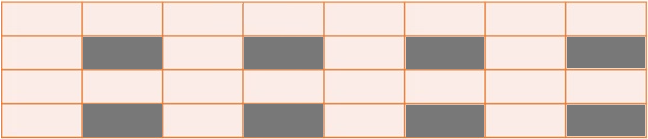
\includegraphics[width=1\textwidth]{Images/diagrams/line_buf_maxp.png}
        \decoRule
        \caption[Line Buffers, Max-Pool]{Line Buffers, Max-Pool: Grey pixels represent which inputs will trigger an output generation.}
        \label{fig: Line Buffers Max-Pool}
\end{figure}

Figure \ref{fig: Line Buffers Max-Pool} demonstrates the Max-Pool layer's uneven output generation, an unavoidable issue of any algorithm with stride greater than one. Following hardware does not operate while there are no data available, which is a problem in a FPGA design, as idle hardware indicates wasted hardware space. By raising the Iteration Interval (II) of the following hardware functions and properly calibrating the size of internal FIFO streams, the constant operation of the entire system is ensured.

The processing component of forward propagation is quite simple, as the output is the highest value in each window. It is important to note that the output's spatial dimensions are two times smaller than those of the input. Even more straightforward is back-propagation, in which the pixels that were the maximums in their windows back-propagate the corresponding error gradients, while the rest back-propagate zero.

\subsubsection{Dense \& Softmax Layers}
The implementations of the dense and Softmax layers are simple and fairly similar. They are made up of two components: matrix multiplication of their inputs and weights and their respective activation function. In back-propagation and gradient calculation, the output error is activated before used as the input, with the input and variable gradients being the outputs.

The most crucial aspect of their design is ensuring that the hardware functions are constantly operating. To accomplish this, a streaming architecture, that reads and writes inputs and outputs serially and only once, is used. Important to note is that the Softmax activation requires all the inputs to be received before calculating any output, meaning that for an example back-propagation can not start until forward propagation is fully completed.

\subsubsection{Pipeline to Generate Gradients} % TODO: find better title
A major advantage of FPGA accelerators is that multiple hardware functions operate simultaneously, if the implemented algorithm allows. This holds true for most of the design. As an example, The first maxpool layer requires four inputs to generate the first output. These inputs have being generated by the first convolutional layer before the training data-point is fully loaded and processed. Thus the first two layers are operating simultaneously. % hardware function operate simutanusly

On the other hand, the Softmax layer, which is the last step of the forward propagation, operates like a barrier. Due to the nature of the algorithm, to produce its feature map, all inputs must first be collected. As a result, for a single training data-point, the forward propagation must be completed before the back propagation begins. % softmax is a barrier

This fact produces numerous issues. First off, for a single data input, not all hardware functions can run concurrently, increasing overall latency. Furthermore, all data that skips layers between forward and back propagation, have to be saved in their entirety since they have already been fully produced before they are used. % problem of the barrier

The pipeline includes three major components, forward propagation, back propagation and gradient calculation. Each one is made up of the relevant hardware functions for the layers of the ANN. The last two components run concurrently, but require the first to finish before they begin. % pipeline

The excessive length of the training pipeline may lead to another problem. When only one input image is used, the first parts of the pipeline have finished, before the last ones have even started. Therefore, hardware functions are idling, resulting in wasted hardware. % problem of lengthy pipeline

\subsubsection{Batching \& Updating Variables}

As described before, not all hardware functions can run concurrently for a single data input. This is mitigated through batching, where while an input runs through back-propagation, the next one is used in forward propagation.

\subsubsection{Data Movement \& Storage}
